
%(BEGIN_QUESTION)
% Copyright 2006, Tony R. Kuphaldt, released under the Creative Commons Attribution License (v 1.0)
% This means you may do almost anything with this work of mine, so long as you give me proper credit

In connecting a pressure transmitter or other pressure-measuring instrument to a process pipe or vessel, there must be some means of ``disconnecting'' the instrument from the pressurized process so that it may be calibrated or removed safely without depressurizing the entire process.  Usually, this feature is provided in the form of an instrument ``manifold,'' consisting of one or more valves between the instrument and the process pipe or vessel.

Take this pressure gauge installation, for example:

$$\includegraphics[width=15.5cm]{i00209x01.eps}$$

Two small valves connect the process vessel to the pressure gauge through a tee fitting, one called the ``block'' and the other called the ``bleed.''  In normal operation, the ``block'' valve remains in the open position and the ``bleed'' valve remains in the closed position.

Suppose you wished to remove this pressure gauge from the process vessel and take it to the instrument shop for re-calibration.  In what sequence would you operate the ``block'' and ``bleed'' valves before loosening the gauge from the tubing?  After the gauge had been calibrated and installed, and you are ready to place it back in service, how would you sequence the opening and closing of the ``block'' and ``bleed'' valves?  {\it Be very careful about the sequence of your steps!}

\underbar{file i00209}
%(END_QUESTION)





%(BEGIN_ANSWER)

Removing the gauge from service:

\begin{itemize}
\item{} Close the ``block'' valve.
\item{} Open the ``bleed'' valve.  If the process fluid is dangerous (toxic, flammable, etc.), be {\it very careful} when ``bleeding'' it to the atmosphere!
\item{} Place lock-out tags on both valve handles to notify operators and technicians of the instrument's removal and pending return.
\item{} Remove the gauge from the piping or tubing.
\end{itemize}

It is very important to place tags on the valve handles as notifiers of your service to the gauge.  Even if these tags do not serve a safety purpose (i.e. it is visually obvious that the ``block'' valve should not be opened when there is no instrument connected to it), they still notify anyone looking for the missing gauge that you are servicing it and will have it returned by a certain time/date.

\vskip 10pt

Placing the gauge back into service:

\begin{itemize}
\item{} Re-attach the gauge to the piping or tubing.
\item{} Remove the lock-out tags on both valve handles.
\item{} Close the ``bleed'' valve.
\item{} Open the ``block'' valve.
\end{itemize}

An added touch of professionalism when opening the ``block'' valve is to not leave it open all the way so that the handle cannot turn any further counterclockwise.  Instead, open it all the way (counterclockwise) until you feel the handle ``stop,'' then turn it back clockwise (in the closing direction) about 1/4 turn.  This helps to prevent the valve from seizing in the fully open position, by backing the valve stem off the reverse seat.  Valves left to sit in the fully open position have a tendency to become ``frozen'' in that position.  The worse thing about a ``frozen'' valve is that you cannot determine what position it is in by feel!

%(END_ANSWER)





%(BEGIN_NOTES)

It would be a good idea to bring some ``Do Not Operate'' tags to class so your students can see exactly what they look like and how to use them.

$$\includegraphics[width=15.5cm]{i00209x02.eps}$$

%INDEX% Safety, isolation valves: block and bleed

%(END_NOTES)


